\chapter{Les limites du Single-Linkage}
\label{chap:limites_single_linkage}

Les deux chapitres précédents confèrent au Single-Linkage une justification précise : dans le cadre euclidien, il reconstruit exactement la hiérarchie des amas de forte densité (pour l'estimateur $1$-NN ; voir \S~\ref{sec:lien_SL_HartiganNN}) ; c'est aussi le seul clustering hiérarchique à répondre à une axiomatique minimale (\Res[res:Axiomatique_Single-Linkage_unique]). 

Mais ces justifications fixent en même temps les limites : dans l'espace euclidien, toute la notion de densité est portée par un unique voisin ; si l'on voit le Single-Linkage comme une application $d\mapsto u$ qui transforme une métrique $d$ en une ultramétrique $u$, il y a la double contrainte imposée par l'ultramétricité et la sous-dominance $u \le d$.


Des versions du Single-Linkage tentant d'intégrer une densité à $K$ voisins ont été proposées. Nous verrons ainsi la filiation du Single-Linkage au \emph{Robust} Single-Linkage (nouvelle distance : la distance de cœur, ou \emph{core distance} en anglais), puis à DBSCAN (ajoutant la bonne idée d'intégrer la frontière des clusters), et enfin à HDBSCAN (qui permet d'obtenir un clustering multi-échelle grâce à la notion d'\emph{excès de masse} ; HDBSCAN procède de plus à un élagage de l'arbre hiérarchique pour une meilleure gestion du bruit).

\Contributions{Ce chapitre constitue encore une revue : le point de départ en est les limites du Single-Linkage ; le point d'arrivée les réponses qui ont été apportées, avec une description plus précise de ce qui est unanimement considéré aujourd'hui comme l'« état-de-l'art » \cite{HDBSCAN2025SOTA, FLASC2025} pour le clustering fondé sur la densité : HDBSCAN \cite{HDBSCAN, HDBSCAN2017}.

Les simples changements de fonction de liaison (remplacer le \emph{Single-} par le \emph{Complete-} ou \emph{Average-}Linkage) apportent plus d'instabilité qu'elles ne règlent de problème (\Res[res:instabilite_complete_linkage]).

Cette revue est critique et, comme nous le verrons dans la partie suivante, HDBSCAN ne répond pas aux objectifs qu'il s'était fixé, savoir : remplacer l'estimateur de densité $1$-NN du Single-Linkage par un $K$-NN. Les utilisateurs réguliers de HDBSCAN savent  d'ailleurs que le paramètre correspondant à ce $K$, \texttt{min\_samples}, produit de mauvais résultats lorsqu'il est trop grand et recommandent souvent en pratique de ne pas excéder une dizaine (même pour des données dépassant les milliers de points). La raison n'en est pas que l'estimateur $K$-NN lisserait trop les clusters, elle est fondamentalement liée à l'approximation de HDBSCAN : la recherche $\min \max$ sur le graphe de voisinage muni de la distance de cœur ne représente plus rien pour $K \gtrsim 10$, et certainement par les véritables amas discrets de forte densité $K$-NN.}



%\Contributions{Dans ce chapitre, nous présentons une analyse critique des limites du Single-Linkage, en détaillant l'effet de chaînage (\emph{chaining effect}) et l'inconsistance démontrée par \textsc{Hartigan} \cite{hartigan81}. Nous montrons pourquoi les simples changements de fonction de liaison (\emph{Complete} ou \emph{Average Linkage}) échouent par instabilité topologique \cite{CarlssonMemoli2010}. Nous décortiquons ensuite les fondements du \emph{Robust Single-Linkage} \cite{RobustSingleLinkage2010}, de DBSCAN \cite{DBSCAN} et de HDBSCAN \cite{HDBSCAN2017}, en soulignant leurs apports indéniables (gestion du bruit, excès de masse) mais aussi leurs contradictions géométriques fondamentales : l'utilisation d'une condition de densité à $K$ voisins combinée à une connectivité d'ordre $1$ (de simples arêtes). Cette analyse prépare le terrain à la partie suivante, où nous introduirons la bonne façon de généraliser l'estimateur $K$-NN \emph{via} les interactions d'ordre supérieur.}


\section{Quand la notion de densité manque : l'effet de chaînage}

L'incapacité du Single-Linkage à séparer correctement certains amas a été relevée très tôt et constitue l'un de ses défauts majeurs en pratique. L'estimation de densité par le plus proche voisin ($1$-NN) étant, par nature, extrêmement sensible aux variations locales ; la présence d'une fine chaîne de points aberrants (\emph{outliers} en anglais) entre deux amas denses et distincts suffit à les agglomérer prématurément dans le dendrogramme. Il manque fondamentalement au Single-Linkage une notion robuste de \emph{densité locale}.

%\paragraph{Le \emph{chaining effect}}

Cette faiblesse est connue sous le nom d'effet de chaînage (ou \emph{chaining effect} en anglais). L'article de \textsc{Carlsson} \& \textsc{Mémoli} \cite{CarlssonMemoli2010} l'illustre en comparant deux topologies diamétralement opposées.

\begin{figure}[!ht]
    \centering
    % Définition du style des points pour ne pas le répéter
    \tikzset{dot/.style={circle, fill=black, inner sep=2pt, outer sep=0pt}}

    % --- (a) Trois points alignés ---
    \begin{subfigure}[b]{0.3\textwidth}
        \centering
        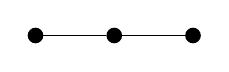
\begin{tikzpicture}[scale=1.]
            % Les points
            \node[dot] (A) at (0,0) {};
            \node[dot] (B) at (1,0) {};
            \node[dot] (C) at (2,0) {};
            
            % Les arêtes (le graphe sous-jacent)
            \draw (A) -- (B) -- (C);
            
            % Labels optionnels pour la distance (décommentez si nécessaire)
            % \node[below, font=\scriptsize] at (0.5,0) {$1$};
            % \node[below, font=\scriptsize] at (1.5,0) {$1$};
        \end{tikzpicture}
        \caption{$\X = \bigl\{x_1,x_2,x_3\bigr\} \subset \mathbb R^1$\label{fig:points_alignes}}
    \end{subfigure}
    \hfill
    % --- (b) Dendrogramme Single-Linkage ---
    \begin{subfigure}[b]{0.3\textwidth}
        \centering
        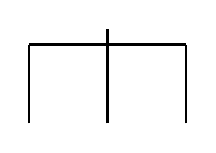
\begin{tikzpicture}[scale=1.]
            % Les feuilles (bas)
            \coordinate (L1) at (0,0);
            \coordinate (L2) at (1,0);
            \coordinate (L3) at (2,0);
            
            % Le niveau de fusion (haut) à hauteur 1
            \coordinate (T1) at (0,1);
            \coordinate (T2) at (1,1.2);
            \coordinate (T3) at (2,1);
            
            % Tracé du dendrogramme (forme de trident car fusion simultanée)
            \draw[thick] (L1) -- (T1);
            \draw[thick] (L2) -- (T2);
            \draw[thick] (L3) -- (T3);
            \draw[thick] (T1) -- (T3); % Barre horizontale
        \end{tikzpicture}
        \caption{Dendrogramme $\theta^\delta$\label{fig:dendrogramme_3points}}
    \end{subfigure}
    \hfill
    % --- (c) Triangle équilatéral ---
    \begin{subfigure}[b]{0.3\textwidth}
        \centering
        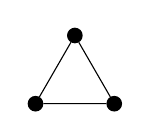
\begin{tikzpicture}[scale=1.]
            % Coordonnées triangle équilatéral de côté 1
            \node[dot] (A) at (0,0) {};
            \node[dot] (B) at (1,0) {};
            \node[dot] (C) at (60:1) {}; % 60 degrés, distance 1
            
            % Les arêtes
            \draw (A) -- (B) -- (C) -- (A);
        \end{tikzpicture}
        \caption{$\mathcal Y = \bigl\{y_1,y_2,y_3\bigl\} \subset \mathbb R^2$\label{fig:triangle_equilateral}}
    \end{subfigure}
    
    \caption{(a) Trois points alignés espacés de $2\delta$. (b) Le dendrogramme résultant pour le Single-Linkage (fusion simultanée à $\delta$). (c) Trois points en triangle équilatéral à distance $2\delta$. %$\phi \colon \X \to \mathcal Y $ est $1$-lipschitzien pour la distance euclidienne.
    }
    \label{fig:chaining_effect}
\end{figure}

Pour modéliser ce phénomène sur des nuages de taille $n$, prenons deux ensembles $\mathcal X = \{x_1, \dots, x_n\}$ et $\mathcal Y = \{y_1, \dots, y_n\}$ munis de deux métriques radicalement différentes (le cas $n=3$ est illustré en \Fig~\ref{fig:chaining_effect}) :
\begin{enumerate}
\item \textbf{La chaîne} (sur $\mathcal X$). La distance est définie par $d_{\mathcal X}(x_i, x_j) = 2\delta|i-j|$. Géométriquement, cela correspond à des points alignés sur une droite et espacés uniformément de $2\delta$.
\item \textbf{La clique dense} (sur $\mathcal Y$). La distance est définie par $d_{\mathcal Y}(y_i,y_j) = 2\delta$ pour toute paire $i \neq j$. Géométriquement, cela correspond aux sommets d'un $(n{-}1)$-simplexe régulier. C'est la structure la plus dense et compacte possible, où tous les nœuds sont équidistants.
\end{enumerate} 

Or, le dendrogramme produit sur $\mathcal{X}$ et sur $\mathcal{Y}$ par le Single-Linkage est rigoureusement identique : il y a fusion simultanée de tous les points au niveau $\delta$. Un algorithme de clustering pertinent devrait pourtant considérer $\mathcal Y$ comme un cluster bien plus significatif et structuré que la chaîne éparse $\mathcal X$.

\subsection{Consistance et inconsistance du Single-Linkage}
C'est \textsc{Hartigan} \cite{hartigan81} qui a montré mathématiquement les conséquences de cet effet de chaînage : la possibilité de formation d'un ``pont'' entre deux clusters rend le Single-Linkage inconsistant en toute dimension $p \ge 2$.
%Ce manque de robustesse géométrique a des conséquences statistiques profondes, formalisées par \textsc{Hartigan} \cite{hartigan81}. En étudiant la convergence du Single-Linkage vers les véritables composantes de haute densité d'une distribution continue, \textsc{Hartigan} a mis en lumière une dichotomie fondamentale liée à la dimension de l'espace $p$.

\begin{Definition}{(\textsc{Hartigan})-Consistance d'un algorithme de clustering hiérarchique \cite{hartigan81}}{hartigan_consistency}
Un algorithme de clustering hiérarchique $\theta$ (\Def[def:dendrogramme]) est dit \emph{consistant} (au sens de \textsc{Hartigan}) si, quels que soient $f$ une fonction de densité suffisamment régulière sur $\mathbb R^p$,  $\lambda > 0$, et $A,B$ deux amas disjoints de forte densité de $f$ au niveau $\lambda$ (et de mesure strictement positive), alors $\theta$ sépare asymptotiquement parfaitement $A$ et $B$ ;  c'est-à-dire qu'avec probabilité tendant vers $1$ lorsque $n\to \infty$, si $\mathcal X_n$ est un nuage de $n$ points tirés i.i.d. selon $f$, il existe $r_n > 0$ tel que $A_n, B_n \in \theta(r_n)$ et $A_n \subset A, B_n \subset B $.
\end{Definition}

\begin{Resultat}{Consistance et inconsistance du Single-Linkage \cite{hartigan81}}{hartigan_consistency}
\begin{itemize}
    \item En dimension $p=1$, l'algorithme de Single-Linkage est un estimateur (\textsc{Hartigan})-{consistant} des amas de forte densité.
    \item En dimension $p \ge 2$, l'algorithme de Single-Linkage est (\textsc{Hartigan})-{inconsistant} pour recouvrer les amas de forte densité. Il n'est que \emph{fractionnellement consistant}.
\end{itemize}
\end{Resultat}

L'explication de cette inconsistance réside dans le phénomène mathématique de {la percolation continue} \cite{MeesterRoy, penrose2003}. En dimension $p \ge 2$, à mesure que le rayon de connexion augmente, des composantes géantes apparaissent presque sûrement. Cependant, avant qu'une composante géante ne parvienne à absorber l'intégralité des points appartenant à son amas de densité, elle \emph{percole} (fusionne) inévitablement avec les composantes géantes voisines \emph{via} des ponts de bruit ($=$ \emph{chaining effect} ; voir \emph{supra} la \Fig[fig:MST_GrapheGeometrique], avec un amas de forte densité central). On ne peut alors espérer recouvrer qu'une \emph{fraction} des points du cluster. 


En dimension $p=1$, ce phénomène de percolation n'existe pas (pour un modèle de \textsc{Poisson} à: l'espace vide maximum sépare toujours parfaitement les modes de la densité.


Nous reviendrons plus amplement sur ce phénomène de percolation dans la partie suivante de ce manuscrit (et notamment au chapitre \ref{sec:chap_percolation}), où nous montrerons comment la théorie nous permet de mesurer la vitesse de percolation (\emph{percolation rate} \cite{BibiVenise, BibiIstambul}) des algorithmes pour quantifier théoriquement cette inconsistance.


\section{Les liaisons dangereuses : Complete- et Average-Linkage}

Pour pallier le défaut structurel du Single-Linkage (le critère très laxiste du «~voisin le plus proche~» entre deux ensembles), l'on pourrait être tenté de recourir à d'autres critères de liaison (\emph{linkage}) lors de l'étape d'agglomération. Citons les deux alternatives historiques les plus célèbres :

\begin{Definition}{Complete-Linkage \cite{Sorensen1948} et Average-Linkage \cite{SokalMichener1958}}{complete_average_linkage}
Soient $C$ et $C'$ deux clusters d'un espace métrique $(\mathcal X, d)$.
\begin{itemize}
    \item \textbf{Complete-Linkage} (liaison complète). La distance entre deux clusters est définie par la distance maximale entre leurs éléments :
    \[
    \boxed{
        d_{\mathrm{CL}}(C, C') = \max_{x \in C, \, y \in C'} d(x,y).
        }
    \]
    \item \textbf{Average-Linkage} (liaison moyenne). La distance est définie par la moyenne des distances entre toutes les paires inter-clusters :
    \[
    \boxed{
        d_{\mathrm{AL}}(C, C') = \frac{1}{|C| |C'|} \sum_{x \in C} \sum_{y \in C'} d(x,y).
        }
    \]
\end{itemize}
\end{Definition}

Empiriquement, ces méthodes tendent à produire des clusters plus compacts (plus ``sphériques'') et évitent l'effet de chaînage. Cependant, elles souffrent d'un défaut théorique rédhibitoire qui les disqualifie pour une analyse topologique rigoureuse.

\begin{Resultat}{Instabilité des Complete- et Average-Linkage \cite{CarlssonMemoli2010}}{instabilite_complete_linkage}
Contrairement au Single-Linkage, les algorithmes de \emph{Complete Linkage} et d'\emph{Average Linkage} sont \emph{instables}. Ils ne satisfont pas la propriété de continuité $1$-lipschitzienne au sens de la distance de \textsc{Gromov-Hausdorff}. Une infime perturbation de l'espace métrique initial peut engendrer des dendrogrammes radicalement différents.
\end{Resultat}

La solution au \emph{chaining effect} ne réside donc pas dans la modification de la fonction de liaison entre ensembles (qui détruit les garanties de stabilité métrique). %, mais plutôt dans une redéfinition de l'espace métrique lui-même et de la manière d'estimer la densité locale.


\section{Introduire la densité locale : le Robust Single-Linkage}
\label{sec:robust_single_linkage}

Pour introduire une notion de densité au Single-Linkage, l'idée naturelle est de substituer l'estimateur de densité du plus proche voison ($1$-NN, responsable de la sensibilité au bruit) par l'estimateur des $K$-Plus Proches Voisins ($K$-NN), cet estimateur ayant de bonnes propriétés de consistance lorsque $K \to \infty$ \cite{BiauDevroye}. 

Cette approche, initialement pressentie par \textsc{Wishart} \cite{RobustSingleLinkage1969}, a été rigoureusement théorisée par \textsc{Chaudhuri} \& \textsc{Dasgupta} \cite{RobustSingleLinkage2010} sous le nom de \emph{Robust Single-Linkage}.

\begin{Definition}{Distance de cœur (\emph{core distance}) \cite{OPTICS1999}}{core_distance}
Soit $\mathcal{X} \subset \mathbb R^p$ un nuage de points de taille $n$ et $K \le n$. La distance de cœur d'un point $x \in \mathcal{X}$, notée $r_K(x)$, est la distance de $x$ à son $K$-ième plus proche voisin dans le nuage :
\[
\boxed{
    r_K(x) = \min \bigl\{ r \ge 0 \bigm| \module{B(x, r) \cap \mathcal{X}} \ge K \bigr\}.
    }
\]
\end{Definition}

La distance de cœur est (à un exposant dimensionnel près) inversement proportionnelle à l'estimateur de densité $K$-NN évalué au point $x$. Pour forcer les points à se regrouper \emph{uniquement} s'ils se trouvent mutuellement dans une région suffisamment dense, \textsc{Chaudhuri} \& \textsc{Dasgupta} \cite{RobustSingleLinkage2010} définissent une nouvelle métrique sur $\mathcal{X}$.

\begin{Definition}{Distance d'atteignabilité mutuelle (\emph{mutual reachability distance}) \cite{RobustSingleLinkage2010}}{mutual_reachability}
La distance d'atteignabilité mutuelle entre deux points $x, x' \in \mathcal{X}$ pour un paramètre $K$ est définie par :
\[
\boxed{
    d_{\mathrm{mreach}, K}(x, x') = \max \bigl\{ r_K(x), r_K(x'), d(x, x') \bigr\}.
    }
\]
\end{Definition}

L'algorithme du {Robust Single-Linkage} consiste alors simplement à appliquer le Single-Linkage classique (l'extraction de l'arbre minimum couvrant), mais en calculant les poids des arêtes avec la distance $d_{\mathrm{mreach}, K}$ au lieu de la distance $d$ originelle de l'espace métrique. 

L'ultramétrique $u^{\mathrm{RSL}}$ induite par le Robust Single-Linkage pouvant, de la même façon que précédemment avec le Single-Linkage, s'exprimer à l'aide d'un $\min \max$ \cite{Draganov2025} (\Res~\ref{res:uRSL} ci-dessous).

\begin{Resultat}{Ultramétrique $u^{\mathrm{RSL}}$ du Robust Single-Linkage exprimée comme un $\min \max$ \cite{Draganov2025}}{uRSL}
Soit $\mathcal X \subset \mathbb R^p$ un nuage $n$ de points, et $K \in \mathbb N^\star, K\le n$ un entier. Soit $d_{\mathrm{mreach}, K}$ la distance d'atteignabilité mutuelle sur $\mathcal X$. Alors l'ultramétrique $u^{\mathrm{RSL_K}}$ induite par le Robust Single-Linkage sur $\mathcal X$ peut s'exprimer ainsi :
\[
\boxed{
    \forall x,x' \in \mathcal X, \ u^{\mathrm{RSL_K}}(x,x') = \min_{\omega : x \rightsquigarrow x'} \max_{(u, v) \in \omega} d_{\mathrm{mreach}, K}(u,v)
    }
    \]
où le minimun est pris sur l'ensemble des chemins $\omega$ de $x$ à $x'$.
\end{Resultat}


\Remarque{Le mécanisme sous-jacent au Robust Single-Linkage est astucieux : pour que deux points soient connectés à un niveau de résolution $r$, il faut non seulement qu'ils soient géométriquement proches, mais également que \emph{chacun d'eux} réside dans une région de haute densité (avoir au moins $K$ voisins dans un rayon $r$, c'est-à-dire $r_K(x) \le r$ et $r_K(y) \le r$).}

\subsection{Critique du Robust Single-Linkage} 
Si cette méthode garantit la consistance asymptotique lorsque $K \to \infty$ \cite{RobustSingleLinkage2010}, à $K$ fixé elle ne permet absolument pas de retrouver les amas de forte densité pour le $K$-NN.
Nous reviendrons beaucoup plus longuement sur ce point dans la partie suivante, et notamment au chapitre \ref{chap:hgp_clusterer}. La façon la plus simple de s'en rendre compte est de prendre la définition $\min \max$ du Robust Single-Linkage : pour un niveau $r>0$ donné, elle garantit que chacun des sommets du meilleur chemin $\omega$ reliant $x$ à $x'$ sont dans des amas de forte densité $K$-NN, mais non pas que le chemin $\omega$ lui-même soit entièrement compris dans un amas de forte densité.
Nous verrons dans la partie suivante que la bonne façon d'introduire l'estimateur $K$-NN, sans briser la topologie des ensembles de niveau, consiste à utiliser des hypergraphes (les complexes de \v{C}ech) et à étendre la notion de connectivité \emph{via} les $K$-polyèdres (\Def[def:k_polyedres]).





\section{L'état de l'art : HDBSCAN}
\label{sec:hdbscan}

\subsection{La gestion explicite de la frontière des clusters : DBSCAN}
\label{sec:dbscan}

%Nous avons déjà mentionné qu'en pratique, le paramètre $K$ du Robust Single-Linkage ne doit pas être pris trop important (et ce pour des raisons profondes d'inexactitude par rapport au modèle des amas de forte densité $K$-NN).
%La gestion de la sensibilité du Robust Single-Linkage au bruit n'en est que plus fragile.
Le Robust Single-Linkage est trop exigeant vis-à-vis d'un point $x \in \mathcal X$ pour qu'il apparaisse dans un cluster (au niveau $r$) : être dans un niveau de forte densité $x \in L_K(r)$. 

Or, comme cela apparaît dans la définition que nous avons posée des amas \emph{discrets} de forte densité (\Def[def:HDC_discret]), un point peut participer à un cluster $C$ (être \emph{couvert} par $C$), sans pour autant appartenir lui-même à $C$. 
C'est toute la gestion délicate de la frontière des clusters et du passage du continu au discret qui apparaît.
Nous verrons dans la partie suivante (au chapitre \ref{sec:chap_percolation}) en comparant les différentes vitesses de percolation que le critère trop fort du Robust Single-Linkage ruine complètement ses performances théoriques.



Il convient de mentionner un algorithme qui a fortement amélioré le Robust Single-Linkage sur ce point précis : DBSCAN, proposé par \textsc{Ester} \etal en 1996 \cite{DBSCAN}.
Par voie de conséquence, DBSCAN a fortement amélioré la gestion du bruit au niveau des frontières, de là son nom : \emph{Density-Based Spatial Clustering of Applications with Noise}. 


DBSCAN catégorise, pour un certain niveau $r$, les points de $\mathcal{X}$ en trois types :

\begin{Definition}{Catégorisation des points dans DBSCAN \cite{DBSCAN}}{dbscan_points}
\begin{enumerate}
    \item \textbf{Points cœurs} (\emph{core points}). Points possédant au moins $K$ voisins dans leur $r$-voisinage ($r_{K}(x) \le r$).
    \item \textbf{Points accessibles} (\emph{reachable points} ou \emph{border points}). Points n'étant pas des cœurs, mais situés dans le $r$-voisinage d'un point cœur. Ils forment la frontière du cluster.
    \item \textbf{Bruit} (\emph{noise} / \emph{outliers}). Tous les autres points, considérés comme isolés.
\end{enumerate}
\end{Definition}
\Remarque{la faiblesse du Robust Single-Linkage consistait à ne pas tenir compte de ce que les auteurs de DBSCAN appellent les points \emph{accessibles}. À un certain niveau $r$, ces points ne font pas partie d'un cœur (ils n'ont pas $K$ voisins), pour autant ils ont participé à la formation d'un amas de forte densité $K$-NN. Ne pas en tenir compte est une erreur. (Erreur qu'on pourra d'ailleurs mesurer dans le chapitre \ref{sec:chap_percolation} grâce à la vitesse de percolation.)
Ces points correspondent à ce que nous avons appelés des points \emph{couverts} par un amas, sans pour autant faire partie d'un amas (voir \Def[def:HDC_discret]).}
% en faire partie (voir \Def[def:HDC_discret]) : 
% \[
% \bigl\{ \bigr\} \eqdef C^\mathrm{discret} \setminus C  .
% \]

L'algorithme connecte ensuite les points cœurs entre eux s'ils sont à une distance mutuelle inférieure à $r$, formant ainsi l'ossature des clusters, auxquels on rattache finalement les points accessibles.


\subsection{HDBSCAN}

Nous avons déjà mentionné qu'en pratique, le paramètre $K$ du Robust Single-Linkage ne doit pas être pris trop important (et ce pour des raisons profondes d'inexactitude par rapport au modèle des amas de forte densité $K$-NN).
La gestion de la sensibilité du Robust Single-Linkage au bruit n'en est que plus fragile.
Cette faiblesse reste en partie vraie pour DBSCAN. De plus, DBSCAN requiert un paramètre de résolution global $r$. Si les données présentent des clusters de densités très variables, aucun rayon $r$ unique ne pourra les extraire simultanément de manière satisfaisante.

HDBSCAN (\emph{Hierarchical DBSCAN}) répond (partiellement) à ces deux limites. \textsc{Campello, Moulavi} \& \textsc{Sander} \cite{HDBSCAN}, puis \textsc{McInnes} \& \textsc{Healy} \cite{HDBSCAN2017}, ont conçu HDBSCAN, algorithme qui est aujourd'hui \emph{la} référence \cite{HDBSCAN2025SOTA, FLASC2025}.



\subsection{Le seuil de percolation (\texttt{min\_cluster\_size}) pour une meilleure gestion du bruit}

La première innovation de HDBSCAN est un élagage systématique de l'arbre hiérarchique. L'algorithme supprime tous les clusters dont la taille est strictement inférieure à un paramètre \texttt{min\_cluster\_size}. Lorsqu'un cluster parent se scinde en deux sous-clusters, on évalue la taille de chaque branche :
\begin{itemize}
    \item Si une seule des deux branches possède suffisamment de points, on considère qu'il ne s'agit pas d'une véritable scission, mais simplement de points de bruit qui se détachent du cluster principal. La branche survivante conserve l'identité de son parent.
    \item Si les deux branches ont une taille supérieur à \texttt{min\_cluster\_size}, la scission est validée et deux nouveaux clusters indépendants naissent.
\end{itemize}


\Remarque{En effectuant cet élagage, les auteurs de HDBSCAN ont introduit un véritable \emph{seuil de percolation} (et ce, sans le formuler explicitement en ces termes). Seules les composantes ``macroscopiques'' sont conservées, éliminant ainsi le bruit des micro-composantes qui apparaissent de manière éphémère.}

\subsection{Un clustering multi-échelle : le critère d'excès de masse (\emph{excess of mass})}

Plutôt que de couper le dendrogramme à une hauteur fixe comme le fait DBSCAN, HDBSCAN introduit un critère de stabilité inspiré des statistiques non paramétriques \cite{MullerSawitzki} pour sélectionner automatiquement les clusters à des échelles variables.

\begin{Definition}{Excès de Masse (\emph{excess of mass}) \cite{HDBSCAN}}{excess_mass}
Pour une fonction de densité continue $f$, l'excès de masse d'un cluster $C$ apparu à un niveau de densité de base $\lambda$ est défini par :
\[
\boxed{
    E(C) = \int_C \bigl(f(x) - \lambda\bigr) \ind{f(x) \ge \lambda} \, \mathrm{d}x.
    }
\]
\end{Definition}

La \Fig~\ref{fig:hdbscan_eom} illustre les excès de masse des différents clusters d'intérêt pour une certaine fonction.

En pratique, cet excès de masse \emph{relatif} (propre à chaque cluster) est très simple à estimer. %Soit un estimateur de densité $\hat{\lambda}_x$ calculé pour chaque point $x \in \mathcal{X}$. 
Si le cluster $C$ commence à exister à partir du seuil de densité $\hat{\lambda}_{\min}$ (moment où il se sépare de son parent) et qu'un point $x \in \mathcal X$ quitte le cluster (devient du bruit ou forme un sous-cluster) à la densité $\hat{\lambda}_x$, l'excès de masse cumulé de $C$ est estimé par :
\[
    \widehat{E}(C) \propto \sum_{x \in C} \bigl(\hat{\lambda}_x - \hat{\lambda}_{\min}\bigr).
\]

HDBSCAN estime la densité en un point $x$ simplement avec l'inverse de la distance à laquelle le point se détache : $\hat{\lambda}_x = 1/r_x$.



\begin{figure}[!h]
    \centering
    \begin{tikzpicture}[scale=0.72, >=latex, font=\small]
        
        % --- DÉFINITION DE LA FONCTION DE DENSITÉ ---
        % Modélisée comme une somme de 3 gaussiennes pour des délimitations mathématiquement parfaites.
        \tikzset{
            declare function={
                f(\x) = 1.8*exp(-pow(\x-1.8, 2)/0.4) + 4.5*exp(-pow(\x-3.5, 2)/0.8) + 2.8*exp(-pow(\x-6.0, 2)/0.6);
            }
        }

        % --- COULEURS PASTEL DES AMAS ---
        \definecolor{c1}{RGB}{142, 198, 155} % Vert
        \definecolor{c2}{RGB}{232, 135, 135} % Rouge
        \definecolor{c3}{RGB}{221, 211, 153} % Jaune
        \definecolor{c4}{RGB}{175, 152, 199} % Violet
        \definecolor{c5}{RGB}{152, 210, 228} % Bleu

        % --- COORDONNÉES EXACTES DES EXTREMA ---
        \def\xone{1.876}   \def\hone{1.941}   % Pic 1
        \def\xtwo{3.499}   \def\htwo{4.501}   % Pic 2
        \def\xthree{5.999} \def\hthree{2.802} % Pic 3
        \def\xsaddleA{2.327} \def\hsaddleA{1.705} % Col entre le Pic 1 et 2 (Minimum local 1)
        \def\xsaddleB{4.899} \def\hsaddleB{0.761} % Col entre le (Pic 1+2) et 3 (Minimum local 2)

        % =========================================================
        % PARTIE GAUCHE : ARBRE HIÉRARCHIQUE SOUS LA COURBE
        % =========================================================
        \begin{scope}[xshift=0cm]
            % Axes
            \draw[->, thick] (0,-0.1) -- (0,5.2) node[left] {$f(x)$};
            \draw[->, thick] (-0.2,0) -- (8.5,0);
            
            % Courbe de la densité
            \draw[thick, blue!80!black] plot[domain=0:8.5, samples=200] (\x, {f(\x)});
            
            % --- Arbre condensé (Lignes hiérarchiques rouges) ---
            
            % C1 et C2 (descendent des pics jusqu'au premier point-selle)
            \draw[very thick, red!80!black] (\xone, \hsaddleA) -- (\xone, \hone);
            \draw[very thick, red!80!black] (\xtwo, \hsaddleA) -- (\xtwo, \htwo);
            
            % Fusion horizontale de C1 et C2
            \draw[very thick, red!80!black] (\xone, \hsaddleA) -- (\xtwo, \hsaddleA);
            
            % C4 (descend EXACTEMENT du premier minimum local jusqu'au deuxième point-selle)
            \draw[very thick, red!80!black] (\xsaddleA, \hsaddleA) -- (\xsaddleA, \hsaddleB);
            
            % C3 (descend du pic 3 jusqu'au deuxième point-selle)
            \draw[very thick, red!80!black] (\xthree, \hsaddleB) -- (\xthree, \hthree);
            
            % Fusion horizontale de C4 et C3
            \draw[very thick, red!80!black] (\xsaddleA, \hsaddleB) -- (\xthree, \hsaddleB);
            
            % C5 (descend EXACTEMENT du deuxième minimum local jusqu'en bas)
            \draw[very thick, red!80!black] (\xsaddleB, \hsaddleB) -- (\xsaddleB, 0);
            
            % Labels avec flèches (centrés sur les nouveaux segments verticaux)
            \draw[<-, shorten <=1pt, semithick] (\xone, {(\hone+\hsaddleA)/2}) -- ++(-0.5, 0) node[left] {$C_1$};
            \draw[<-, shorten <=1pt, semithick] (\xtwo, {(\htwo+\hsaddleA)/2}) -- ++(-0.5, 0) node[left] {$C_2$};
            \draw[<-, shorten <=1pt, semithick] (\xsaddleA, {(\hsaddleA+\hsaddleB)/2}) -- ++(-0.5, 0) node[left] {$C_4$};
            \draw[<-, shorten <=1pt, semithick] (\xthree, {(\hthree+\hsaddleB)/2}) -- ++(-0.5, 0) node[left] {$C_3$};
            \draw[<-, shorten <=1pt, semithick] (\xsaddleB, {\hsaddleB/2}) -- ++(-0.5, 0) node[left] {$C_5$};
        \end{scope}

        % =========================================================
        % PARTIE DROITE : EXCÈS DE MASSE ET PARTITIONNEMENT
        % =========================================================
        \begin{scope}[xshift=9.8cm]
            % Axes
            \draw[->, thick] (0,-0.1) -- (0,5.2) node[left] {$f(x)$};
            \draw[->, thick] (-0.2,0) -- (8.5,0);
            
            % Définition du chemin englobant l'intégralité de la courbe
            \def\fillpath{ (0,0) -- plot[domain=0:8.5, samples=200] (\x, {f(\x)}) -- (8.5,0) -- cycle }
            
            % Peinture par couches superposées (du fond vers l'avant) garantissant zéro trou
            \fill[c5] \fillpath;
            
            \begin{scope} \clip (-0.1, \hsaddleB) rectangle (9, 6);
                \fill[c4] \fillpath; \end{scope}
            
            \begin{scope} \clip (\xsaddleB, \hsaddleB) rectangle (9, 6);
                \fill[c3] \fillpath; \end{scope}
            
            \begin{scope} \clip (-0.1, \hsaddleA) rectangle (\xsaddleB, 6);
                \fill[c2] \fillpath; \end{scope}
            
            \begin{scope} \clip (-0.1, \hsaddleA) rectangle (\xsaddleA, 6);
                \fill[c1] \fillpath; \end{scope}
            
            % Lignes de séparation blanches horizontales
            \begin{scope}
                \clip \fillpath;
                \draw[white, line width=1.5pt] (-0.1, \hsaddleB) -- (9, \hsaddleB);
                \draw[white, line width=1.5pt] (-0.1, \hsaddleA) -- (\xsaddleB, \hsaddleA);
            \end{scope}
            
            % Retracer le contour de la densité par-dessus les aires pour des bords parfaits
            \draw[thick, blue!80!black] plot[domain=0:8.5, samples=200] (\x, {f(\x)});
            
            % Légende des amas en haut à droite
            \begin{scope}[shift={(7.2, 4.6)}]
                % Fond semi-transparent adoucissant la collision avec la courbe
                \fill[white, rounded corners=2pt, fill opacity=0.8] (-0.2, 0.4) rectangle (1.2, -1.8);
                
                \fill[c1] (0, 0) rectangle (0.4, 0.2);
                \node[right] at (0.4, 0.1) {$C_1$};
                
                \fill[c2] (0, -0.4) rectangle (0.4, -0.2);
                \node[right] at (0.4, -0.3) {$C_2$};
                
                \fill[c3] (0, -0.8) rectangle (0.4, -0.6);
                \node[right] at (0.4, -0.7) {$C_3$};
                
                \fill[c4] (0, -1.2) rectangle (0.4, -1.0);
                \node[right] at (0.4, -1.1) {$C_4$};
                
                \fill[c5] (0, -1.6) rectangle (0.4, -1.4);
                \node[right] at (0.4, -1.5) {$C_5$};
            \end{scope}
        \end{scope}
        
    \end{tikzpicture}
    \caption{Illustration du critère d'excès de masse de l'algorithme HDBSCAN. \`A gauche~: l'arbre hiérarchique. À droite~: les composantes connexes des ensembles de niveau de la densité délimitant l'excès de masse \emph{relatif}, c'est-à-dire propre à chaque amas $C_i$.}
    \label{fig:hdbscan_eom}
\end{figure}


Pour extraire le partitionnement final, l'algorithme parcourt l'arbre condensé de bas en haut. À chaque nœud parent divisé en plusieurs enfants, on compare son excès de masse empirique $\widehat{E}(C)$ avec la somme des stabilités de ses enfants. On définit ainsi récursivement la \emph{stabilité} $\tilde{E}(C)$ d'un cluster par :
\[
    \tilde{E}(C) = \begin{cases}
        \widehat{E}(C) & \text{si } C \text{ est une feuille,} \\
        \max \left( \widehat{E}(C), \displaystyle\sum_{C_i \in \text{Fils}(C)} \tilde{E}(C_i) \right) & \text{sinon.}
    \end{cases}
\]
Si la stabilité des enfants est supérieure, la scission est validée et on parcourt les n\oe uds enfants. Sinon, le parent est sélectionné comme un cluster unique et robuste ($\tilde{E}(C) = \widehat{E}(C)$). Cette optimisation permet à HDBSCAN d'extraire des clusters à des niveaux de densité très différents.

La Figure~\ref{fig:hdbscan_eom} illustre ce processus, où l'excès de masse relatif $\widehat{E}$ correspond à l'aire des régions colorées. L'algorithme initialise les feuilles avec leurs aires respectives : $\tilde{E}(\textcolor{c1!80!black}{\mathbf{C_1}})$, $\tilde{E}(\textcolor{c2!80!black}{\mathbf{C_2}})$ et $\tilde{E}(\textcolor{c3!80!black}{\mathbf{C_3}})$. En remontant au nœud parent $\textcolor{c4!80!black}{\mathbf{C_4}}$, la somme des aires \textbf{\textcolor{c1!80!black}{verte}} et \textbf{\textcolor{c2!80!black}{rouge}} s'avère supérieure à l'aire \textbf{\textcolor{c4!80!black}{violette}} du parent : la scission est donc conservée. Le processus s'achève à la racine $\textcolor{c5!80!black}{\mathbf{C_5}}$, où la somme des stabilités consolidées des branches ($\tilde{E}(\textcolor{c4!80!black}{\mathbf{C_4}}) + \tilde{E}(\textcolor{c3!80!black}{\mathbf{C_3}})$) dépasse l'aire \textbf{\textcolor{c5!80!black}{bleue}} de la base. Le partitionnement final renvoyé par HDBSCAN sur cet exemple est donc : $\textcolor{c1!80!black}{\mathbf{C_1}}$, $\textcolor{c2!80!black}{\mathbf{C_2}}$ et $\textcolor{c3!80!black}{\mathbf{C_3}}$.



\subsection{Les limites de l'approche : le paradoxe du choix de $K$}

Puisque HDBSCAN vise à utiliser l'estimateur $K$-NN, la logique statistique dicterait que plus $K$ est grand, plus l'estimation de densité est consistante et lisse, et meilleurs devraient être les résultats. 

Or, en pratique, choisir un $K$ (\emph{via} le paramètre \texttt{min\_samples}) supérieur à une dizaine dégrade rapidement les performances géométriques de l'algorithme, noyant les structures dans le bruit. 
Nous expliquerons théoriquement ce phénomène dans la partie suivante. 
% Si l'on analyse le modèle sous l'angle du taux de percolation $v^K$ (le ratio entre le rayon d'apparition de la composante géante et le rayon où elle absorbe presque tous les points), on démontre que la borne théorique évolue comme :
% \[
%     v^K = 1 - \mathcal{O}\left( \frac{1}{\sqrt{K}} \right).
% \]

% \begin{figure}[!ht]
%     \centering
%     \fbox{\parbox{0.8\textwidth}{\centering \vspace{0.5cm}\textit{[Insérer ici la Figure 5 de l'article SRC \cite{BibiVenise} : "Theoretical bound and exact value of the discretized RSL percolation rate", montrant la convergence en $1/\sqrt{K}$.]}\vspace{0.5cm}}}
%     \caption{Taux de percolation du Robust Single-Linkage discrétisé en fonction de $K$. La convergence vers un taux optimal ($v=1$) est si lente que le compromis $K=10$ est souvent le seul viable.}
%     \label{fig:percolation_rate_K}
% \end{figure}

% La convergence en $1/\sqrt{K}$ est si lente que le gain théorique apporté par un grand $K$ est annihilé par le défaut topologique du Robust Single-Linkage.



\Synthese{L'évolution historique du Single-Linkage vers le Robust Single-Linkage et HDBSCAN illustre le besoin d'intégrer une densité des $K$ plus proches voisins, indispensable pour lutter contre l'inconsistance du modèle (l'effet de chaînage dû à la percolation) et isoler efficacement le bruit.

Toutefois, en dépit de ses bonnes heuristiques d'extraction (condensation de l'arbre hiérarchique \emph{via} \texttt{min\_cluster\_size} et excès de masse), HDBSCAN repose fondamentalement sur le {Robust Single-Linkage}. Cet algorithme n'évalue que ponctuellement la densité (en les points $x \in \mathcal X$) et construit un graphe sur $\mathcal X$ qui n'a pas de raison de refléter les amas de forte densité lorsque $K\ge2$. C'est pourquoi, en pratique, augmenter le paramètre $K$ (\texttt{min\_samples}) dégrade rapidement les performances géométriques de l'algorithme (un compromis faible comme $K=10$ est souvent privilégié). %La recherche d'une composante connexe sur de simples arêtes ne représente plus fidèlement la topologie d'un estimateur $K$-NN.

Comme nous le démontrerons dans la partie suivante, la manière mathématiquement exacte d'introduire l'estimateur $K$-NN exige de généraliser la notion même de connexité. En passant aux hypergraphes (\emph{via} les complexes de \v{C}ech) et en introduisant des interactions d'ordre supérieur avec les $K$-polyèdres, nous rétablirons l'exactitude topologique perdue, tout en fournissant un cadre rigoureux pour analyser théoriquement les performances de ces algorithmes en recourant à la théorie de la percolation.}